
\de{ĐỀ THI HỌC KỲ I NĂM HỌC 2022-2023}{Trường THPT Ngô Gia Tự - Phú Yên}
\begin{center}
	\textbf{PHẦN 1 - TRẮC NGHIỆM}
\end{center}
\Opensolutionfile{ans}[ans/ans]
%Câu 1...........................
\begin{ex}%[0D1B1-3]%[Dự án đề kiểm tra HKI NH22-23- Mui Doan]%[Ngô Gia Tự-Phú Yên]
	Cho mệnh đề \lq\lq $\exists x \in\mathbb{Z}, x^2-5x-6 > 0$\rq\rq. Mệnh đề phủ định sẽ là
	\choice
	{\True $\forall x\in\mathbb{Z}, x^2-5x-6\leq 0$}
	{$\forall x\in\mathbb{Z}, x^2-5x-6< 0$}
	{$\forall x\in\mathbb{Z}, x^2-5x6\geq 0$}
	{$\forall x\in\mathbb{R}, x^2-5x-6>0 0$}
	\loigiai{
	Mệnh đề phủ định sẽ là 	$\forall x\in\mathbb{Z}, x^2-5x-6\leq 0$.
	}
\end{ex}
%Câu 2...........................
\begin{ex}%[0D1Y2-2]%[Dự án đề kiểm tra HKI NH22-23- Mui Doan]%[Ngô Gia Tự-Phú Yên]
	Trong các khẳng định sau, khẳng định nào sai?
	\choice
	{\True $\mathbb{Q}\subset \mathbb{Z}$}
	{$\mathbb{Q}\subset \mathbb{R}$}
	{$\mathbb{Z}\subset \mathbb{R}$}
	{$\mathbb{N}\subset \mathbb{Q}$}
	\loigiai{
	Khẳng định nào sai là	$\mathbb{Q}\subset \mathbb{Z}$.
	}
\end{ex}
%Câu 3...........................
\begin{ex}%[0H3Y1-3]%[Dự án đề kiểm tra HKI NH22-23- Mui Doan]%[Ngô Gia Tự-Phú Yên]
	Trong mặt phẳng tọa độ $Oxy$, tọa độ $\overrightarrow{u}=3\overrightarrow{i}-2\overrightarrow{j}$ là
	\choice
	{$(2;-3)$}
	{$(3;2) $}
	{$(2;3)$}
	{\True $(3;-2)$}
	\loigiai{
	Tọa độ $\overrightarrow{u}=3\overrightarrow{i}-2\overrightarrow{j}$ là	$(3;-2)$.
	}
\end{ex}
%Câu 4...........................
\begin{ex}%[0D2Y2-1]%[Dự án đề kiểm tra HKI NH22-23- Mui Doan]%[Ngô Gia Tự-Phú Yên]
	Hệ bất phương trình nào sau đây là hệ bất phương trình bậc nhất hai ẩn?
	\choice
	{$\heva{&x+y+z>1\\&-x+2y<3}$}
	{\True $\heva{&x+3y>-2\\&-x+y<1}$}
	{$\heva{&x^2+y>2\\&-x+2y<1}$}
	{$\heva{&x+2xy+y>5\\&-x+3xy<3}$}
	\loigiai{
	Hệ bất phương trình bậc nhất hai ẩn là	$\heva{&x+3y>-2\\&-x+y<1}$.
	}
\end{ex}
%Câu 5...........................
\begin{ex}%[0H2Y2-1]%[Dự án đề kiểm tra HKI NH22-23- Mui Doan]%[Ngô Gia Tự-Phú Yên]
	Rút gọn biểu thức $\overrightarrow{EF} - \overrightarrow{GF} + \overrightarrow{GH}$ ta được kết quả
	\choice
	{$\overrightarrow{EG}$}
	{$\overrightarrow{FH}$}
	{$\overrightarrow{0}$}
	{\True $\overrightarrow{EH}$}
	\loigiai{
	Ta có 	$\overrightarrow{EF} - \overrightarrow{GF} + \overrightarrow{GH}=\overrightarrow{EF} + \overrightarrow{FG} + \overrightarrow{GH}=\overrightarrow{EH}$
	}
\end{ex}
%Câu 6...........................
\begin{ex}%[0X1B3-2]%[Dự án đề kiểm tra HKI NH22-23- Mui Doan]%[Ngô Gia Tự-Phú Yên]
	Trung vị của mẫu số liệu $4$; $6$; $7$; $6$; $8$; $7$; $5$; $5$; $4$ là
	\choice
	{\True $6$}
	{$7$}
	{$8$}
	{$5$}
	\loigiai{
	Sắp xếp dãy số theo thứ tự không giảm ta được 	$4$;~ $4$;~ $5$;~ $5$;~ $6$;~ $6$; $7$;~ $7$;~ $8$.\\
	Trung vị của mẫu số liệu là $6$.
	}
\end{ex}
%Câu 7...........................
\begin{ex}%[0H1B2-1]%[Dự án đề kiểm tra HKI NH22-23- Mui Doan]%[Ngô Gia Tự-Phú Yên]
	Cho tam giác $ABC$ có $\widehat{BAC} = 30^\circ$, $BC=3$. Độ dài bán kính đường tròn ngoại tiếp tam giác $ABC$ bằng
	\choice
	{$R=\dfrac{3}{2}$}
	{$R=6$}
	{\True $R=3$}
	{$R=1$}
	\loigiai{
	Theo định lí sin ta có $R=\dfrac{BC}{2\sin \widehat{BAC}}=\dfrac{3}{2\sin 30^\circ}=3$.	
	}
\end{ex}
%Câu 8...........................
\begin{ex}%[0H3Y1-3]%[Dự án đề kiểm tra HKI NH22-23- Mui Doan]%[Ngô Gia Tự-Phú Yên]
	Trong mặt phẳng tọa độ $Oxy$, cho hai điểm $M(-2;3)$, $N(3; 4)$. Tọa độ của $\overrightarrow{MN}$ là
	\choice
	{$(2;5)$}
	{$7$}
	{$(-3;-1)$}
	{\True$(5;1)$}
	\loigiai{
	Ta có 	$\overrightarrow{MN}=(5;1)$.
	}
\end{ex}
%Câu 9...........................
\begin{ex}%[0H1B2-2]%[Dự án đề kiểm tra HKI NH22-23- Mui Doan]%[Ngô Gia Tự-Phú Yên]
	Cho tam giác ABC có $AB=3$, $AC= 2\sqrt{3}$, $A=60^\circ$. Diện tích của tam giác $ABC$ bằng
	\choice
	{$\dfrac{3}{2}$}
	{$\dfrac{9}{4}$}
	{\True $\dfrac{9}{2}$}
	{$9$}
	\loigiai{
	Ta có $S_{\triangle ABC}=\dfrac{1}{2}\cdot AB\cdot AC\cdot \sin A= \dfrac{1}{2}\cdot 3\cdot 2\sqrt{3}\cdot \sin 60^\circ=\dfrac{9}{2}$.	
	}
\end{ex}
%Câu 10...........................
\begin{ex}%[0H1B1-2]%[Dự án đề kiểm tra HKI NH22-23- Mui Doan]%[Ngô Gia Tự-Phú Yên]
	Cho góc $\alpha,~ (0^\circ <\alpha < 180^\circ)$ thỏa mãn $\cos \alpha =\dfrac{3}{4}$. Khẳng định nào sau đây là đúng ?
	\choice
	{\True $\sin\alpha=\dfrac{\sqrt{7}}{4}$}
	{$\sin\alpha=\dfrac{1}{4}$}
	{$\sin\alpha=\dfrac{7}{4}$}
	{$\sin\alpha=\dfrac{7}{16}$}
	\loigiai{
	Ta có $\sin^2\alpha=1-\cos^2\alpha= \dfrac{7}{16}\Rightarrow \sin\alpha=\dfrac{\sqrt{7}}{4}$ (vì $0^\circ <\alpha < 180^\circ)$.
	}
\end{ex}
%Câu 11...........................
\begin{ex}%[0H1B1-2]%[Dự án đề kiểm tra HKI NH22-23- Mui Doan]%[Ngô Gia Tự-Phú Yên]
	Cho góc $\alpha, ~(0^\circ <\alpha < 180^\circ)$ thỏa mãn $\cot \alpha=4$. Tính giá trị biểu thức $$P=\dfrac{\sin\alpha-3\cos\alpha}{2\sin\alpha+\cos\alpha}.$$
	\choice
	{\True $P=-\dfrac{11}{6}$}
	{$P=\dfrac{11}{6}$}
	{$P=\dfrac{13}{6}$}
	{$P=1$}
	\loigiai{
	Ta có 	
	\allowdisplaybreaks
	\begin{align*}
		P&=\dfrac{\sin\alpha-3\cos\alpha}{2\sin\alpha+\cos\alpha}
		\\
		&=\dfrac{1-3\cot\alpha}{2+\cot\alpha}
		\\
		&=\dfrac{1-3\cdot 4}{2+4}
		\\
		&=-\dfrac{11}{6}.
	\end{align*}
	}
\end{ex}
%Câu 12...........................
\begin{ex}%[0H1B2-1]%[Dự án đề kiểm tra HKI NH22-23- Mui Doan]%[Ngô Gia Tự-Phú Yên]
	Cho tam giác $ABC$	có cạnh	$AB=a$;	$AC = a\sqrt{3}$;	$BC = a\sqrt{7}$. Tính góc $\widehat{BAC}$.
	\choice
	{\True $30^\circ$}
	{$150^\circ$}
	{$60^\circ$}
	{$120^\circ$}
	\loigiai{
	Theo định lí cosin	ta có 
	\allowdisplaybreaks
	\begin{align*}
		\cos \widehat{BAC}&=\dfrac{AB^2+AC^2-BC^2}{2\cdot AB\cdot AC}
		\\
		&=\dfrac{a^2+\left(a\sqrt{3}\right)^2-\left(a\sqrt{7}\right)^2}{2\cdot a\cdot a\sqrt{3}}
		\\
		&=\dfrac{\sqrt{3}}{2}.
	\end{align*}
	Suy ra $\widehat{BAC}=30^\circ$.
	}
\end{ex}
%Câu 13...........................
\begin{ex}%[0D1B3-2]%[Dự án đề kiểm tra HKI NH22-23- Mui Doan]%[Ngô Gia Tự-Phú Yên]
	Cho tập hợp $A=\{x\in\mathbb{Z},-2<x < 6\}$ và $B=\{x\in\mathbb{N},-4 <x <5\}$. Tập hợp $A\cap B$ có bao nhiêu phần tử?
	\choice
	{$7$}
	{$4$}
	{$6$}
	{\True $5$}
	\loigiai{
	Ta có 	$A=\{-1;0;1;2;3;4;5\}$, $B=\{-3;-2;-1;0;1;2;3;4\}$.\\
	Suy ra $A\cap B=\{0;1;2;3;4\}$.\\
	 Tập hợp $A\cap B$ có $5$ nhiêu phần tử.
	}
\end{ex}
%Câu 14...........................
\begin{ex}%[0D2Y1-1]%[Dự án đề kiểm tra HKI NH22-23- Mui Doan]%[Ngô Gia Tự-Phú Yên]
	Cặp số $(x;y)$ nào sau đây là nghiệm của bất phương trình $x - 3y > 4$?
	\choice
	{$(1;-1)$}
	{\True $(1;-2)$}
	{$(0;5)$}
	{$(-3;2)$}
	\loigiai{
		\begin{itemize}
			\item Ta có $1-3\cdot (-1)>4$ sai nên $(1;-1)$ không là nghiệm của $x - 3y > 4$.
			\item Ta có $1-3\cdot (-2)>4$ đúng nên $(1;-2)$ là nghiệm của $x - 3y > 4$.
			\item Ta có $0-3\cdot 5>4$ sai nên $(0;5)$ không là nghiệm của $x - 3y > 4$.
			\item Ta có $-3-3\cdot 2>4$ sai nên $(-3;2)$ không là nghiệm của $x - 3y > 4$.
		\end{itemize}
	}
\end{ex}
%Câu 15...........................
\begin{ex}%[0D2B1-1]%[Dự án đề kiểm tra HKI NH22-23- Mui Doan]%[Ngô Gia Tự-Phú Yên]
	Với giá trị nào của $m$, cặp số $(3;-2)$ là một nghiệm của bất phương trình $$(m -1)x - y \geq 2?$$
	\choice
	{$m<-1$}
	{\True $m\geq 1$}
	{$m\leq 1$}
	{$m>-3 $}
	\loigiai{
	Ta có $(3;-2)$ là một nghiệm của bất phương trình $(m -1)x - y \geq 2$ nếu $$(m-1)\cdot 3-(-2)\geq 2\Leftrightarrow m\geq 1. $$	
	}
\end{ex}
%Câu 16...........................
\begin{ex}%[0H2B2-3]%[Dự án đề kiểm tra HKI NH22-23- Mui Doan]%[Ngô Gia Tự-Phú Yên]
	Cho đoạn thẳng $AB$. Gọi $M$ là một điểm trên đoạn thẳng $AB$ sao cho $AB = 3AM$. Khẳng định nào sau đây đúng?
	\choice
	{$\overrightarrow{MA}=-2\overrightarrow{MB}$}
	{$\overrightarrow{MA}=3\overrightarrow{MB}$}
	{\True $\overrightarrow{MA}=-\dfrac{1}{2}\overrightarrow{MB}$}
	{$\overrightarrow{MA}=\dfrac{1}{3}\overrightarrow{MB}$}
	\loigiai{
	Vì $M$ là một điểm trên đoạn thẳng $AB$ sao cho $AB = 3AM$ nên 	$\overrightarrow{MA}=-\dfrac{1}{2}\overrightarrow{MB}$.
	}
\end{ex}
%Câu 17...........................
\begin{ex}%[0H1B1-2]%[Dự án đề kiểm tra HKI NH22-23- Mui Doan]%[Ngô Gia Tự-Phú Yên]
	Khẳng định nào sau đây sai?
	\choice
	{\True $\cos 45^\circ+\cos 135^\circ=\sqrt{2}$}
	{$\tan 45^\circ\cdot\cot 45^\circ=1$}
	{$\sin 45^\circ+\cos 45^\circ=\sqrt{2}$}
	{$\cot 45^\circ+\cot 135^\circ=0$}
	\loigiai{
	Ta có 	$\cos 45^\circ+\cos 135^\circ=\dfrac{\sqrt{2}}{2}-\dfrac{\sqrt{2}}{2}=0$.\\
	Vậy $\cos 45^\circ+\cos 135^\circ=\sqrt{2}$ là khẳng định sai.
	}
\end{ex}
%Câu 18...........................
\begin{ex}%[0H2B4-2]%[Dự án đề kiểm tra HKI NH22-23- Mui Doan]%[Ngô Gia Tự-Phú Yên]
	Cho tam giác $ABC$ cân tại $B$ có cạnh $AB=4$ và $\overrightarrow{AB}\cdot \overrightarrow{BC}=-8$. Tính góc $\widehat{BAC}$.
	\choice
	{\True $60^\circ $}
	{$120^\circ $}
	{$45^\circ $}
	{$30^\circ $}
	\loigiai{
	Vì 	tam giác $ABC$ cân tại $B$ nên $AB=BC=4$.\\
	Ta có 
	\allowdisplaybreaks
	\begin{align*}
		&\overrightarrow{AB}\cdot \overrightarrow{BC}=-8
		\\
		\Leftrightarrow\,\,& \overrightarrow{BA}\cdot \overrightarrow{BC}=8
		\\
		\Leftrightarrow\,\,& AB\cdot BC\cdot \cos \widehat{BAC}=8
		\\
		\Leftrightarrow\,\,& 4\cdot 4\cdot \cos \widehat{BAC}=8
		\\
		\Leftrightarrow\,\,& \cos \widehat{BAC}=\dfrac{1}{2}
		\\
		\Leftrightarrow\,\,&  \widehat{BAC}=60^\circ.
	\end{align*}
	}
\end{ex}
%Câu 19...........................
\begin{ex}%[0X1Y3-5]%[Dự án đề kiểm tra HKI NH22-23- Mui Doan]%[Ngô Gia Tự-Phú Yên]
	Chọn khẳng định sai trong các khẳng định sau khi nói về một mẫu số liệu.
	\choice
	{Trong một mẫu số liệu, số trung vị là duy nhất}
	{Trong một mẫu số liệu, tứ phân vị dưới là duy nhất}
	{\True Trong một mẫu số liệu, mốt là duy nhất}
	{Trong một mẫu số liệu, số trung bình là duy nhất}
	\loigiai{
	Khẳng định sai  là	\lq\lq Trong một mẫu số liệu, mốt là duy nhất\rq\rq.
	}
\end{ex}
%Câu 20...........................
\begin{ex}%[0D1Y1-2]%[Dự án đề kiểm tra HKI NH22-23- Mui Doan]%[Ngô Gia Tự-Phú Yên]
	Mệnh đề nào sau đây là mệnh đề đúng?
	\choice
	{Số	$\pi$	là một số hữu tỷ}
	{Số	$\pi$ là một số nguyên}
	{\True Số	$\pi$ là một số vô tỷ}
	{Số	$\pi$ là một số tự nhiên}
	\loigiai{
	 Mệnh đề đúng là \lq\lq Số	$\pi$ là một số vô tỷ\rq\rq.
	}
\end{ex}
%Câu 21...........................
\begin{ex}%[0H2B2-5]%[Dự án đề kiểm tra HKI NH22-23- Mui Doan]%[Ngô Gia Tự-Phú Yên]
	Cho tam giác đều $ABC$ cạnh bằng $2a$. Độ dài của véc-tơ $\overrightarrow{AB} + \overrightarrow{BC}$ bằng
	\choice
	{\True $2a$}
	{$0$}
	{$a$}
	{$3a$}
	\loigiai{
	Ta có $\left|\overrightarrow{AB} + \overrightarrow{BC}\right|=\left|\overrightarrow{AC}\right|=2a$.	
	}
\end{ex}
%Câu 22...........................
\begin{ex}%[0D1Y1-1]%[Dự án đề kiểm tra HKI NH22-23- Mui Doan]%[Ngô Gia Tự-Phú Yên]
	Phát biểu nào sau đây là một mệnh đề?
	\choice
	{Bạn nên học hành chăm chỉ}
	{Thời tiết hôm nay thật đẹp !}
	{Bây giờ là mấy giờ?}
	{\True Số $4$ là một số chính phương}
	\loigiai{
	Mệnh đề là 	\lq\lq Số $4$ là một số chính phương\rq\rq.
	}
\end{ex}
%Câu 23...........................
\begin{ex}%[0D1B3-2]%[Dự án đề kiểm tra HKI NH22-23- Mui Doan]%[Ngô Gia Tự-Phú Yên]
	Cho các tập hợp $A=(5;+\infty)$ và $B=[0;10]$. Số phần tử là số nguyên của tập $B\setminus A$ là
	\choice
	{Vô số}
	{\True $6$}
	{$7$}
	{$8$}
	\loigiai{
	Ta có $B\setminus A=[0;5]$.\\
	Số phần tử là số nguyên của tập $B\setminus A$ là	$6$.
	}
\end{ex}
%Câu 24...........................
\begin{ex}%[0D1Y2-3]%[Dự án đề kiểm tra HKI NH22-23- Mui Doan]%[Ngô Gia Tự-Phú Yên]
	Dùng các kí hiệu khoảng, đoạn, nửa khoảng để viết lại tập hợp $A=\{x \in\mathbb{R}\,|\, -5 <x < 8\}$.
	\choice
	{$(-5;8]$}
	{$[-5;8)$}
	{$[-5;8]$}
	{\True $(-5;8)$}
	\loigiai{
	Ta có 	$A=(-5;8)$.
	}
\end{ex}
%Câu 25...........................
\begin{ex}%[0H3B2-4]%[Dự án đề kiểm tra HKI NH22-23- Mui Doan]%[Ngô Gia Tự-Phú Yên]
	Trong mặt phẳng tọa độ $Oxy$, cho véc-tơ $\overrightarrow{u}=(1;4)$, $\overrightarrow{v} = (x;2)$. Giá trị của $x$ để $\overrightarrow{u}$ và $\overrightarrow{v}$ vuông góc nhau là
	\choice
	{$x=4$}
	{$x=8$}
	{\True $x=-8$}
	{$x=-\dfrac{1}{2}$}
	\loigiai{
	Ta có 	$\overrightarrow{u}\perp\overrightarrow{v}\Leftrightarrow\overrightarrow{u}\cdot\overrightarrow{v}=0\Leftrightarrow x+8=0\Leftrightarrow x=-8$. 
	}
\end{ex}
%Câu 26...........................
\begin{ex}%[0H3B2-1]%[Dự án đề kiểm tra HKI NH22-23- Mui Doan]%[Ngô Gia Tự-Phú Yên]
	Cho hai véc-tơ $\overrightarrow{a}$ và $\overrightarrow{b}$ thỏa mãn $\left|\overrightarrow{a}\right|=2$, $\left|\overrightarrow{b}\right| = 5$ và $\cos \left(\overrightarrow{a},\overrightarrow{b}\right)=\dfrac{2}{5}$. Tính tích vô hướng $\overrightarrow{a}\cdot \overrightarrow{b}$.
	\choice
	{\True $\overrightarrow{a}\cdot \overrightarrow{b}=4$}
	{$\overrightarrow{a}\cdot \overrightarrow{b}=\dfrac{2}{5}$}
	{$\overrightarrow{a}\cdot \overrightarrow{b}=\dfrac{4}{5}$}
	{$\overrightarrow{a}\cdot \overrightarrow{b}=0$}
	\loigiai{
	Ta có 	$\overrightarrow{a}\cdot \overrightarrow{b}=\left|\overrightarrow{a}\right|\cdot \left| \overrightarrow{b}\right|\cdot \cos \left(\overrightarrow{a},\overrightarrow{b}\right)=2\cdot 5\cdot \dfrac{2}{5}=4$.
	}
\end{ex}
%Câu 27...........................
\begin{ex}%[0H1B3-1]%[Dự án đề kiểm tra HKI NH22-23- Mui Doan]%[Ngô Gia Tự-Phú Yên]
	Cho tam giác $ABC$ có $AB = 7$, $AC = 9$ và đường trung tuyến $AM=7$. Tính chu vi của tam giác $ABC$.
	\choice
	{$1$}
	{$\sqrt{2}$}
	{$30$}
	{\True $24$}
	\loigiai{
	Ta có 
	\allowdisplaybreaks
	\begin{align*}
		&AM^2=\dfrac{2(AB^2+AC^2)-BC^2}{4}
		\\
		\Leftrightarrow\,\,& 7^2= \dfrac{2(7^2+9^2)-BC^2}{4}
		\\
		\Leftrightarrow\,\,& BC^2=2(9^2-7^2)=64
		\\
		\Leftrightarrow\,\,& BC=8.
	\end{align*}	
	Chu vi của tam giác $ABC$ là $7+9+8=24$.
	}
\end{ex}
%Câu 28...........................
\begin{ex}%[0H3B2-3]%[Dự án đề kiểm tra HKI NH22-23- Mui Doan]%[Ngô Gia Tự-Phú Yên]
	Trong mặt phẳng tọa độ $Oxy$, cho $\triangle ABC$ biết $A(0;8)$, $B(3;1)$, $C(-7;5)$. Khi đó $\triangle ABC$ là
	\choice
	{\True Tam giác vuông cân tại $A$}
	{Tam giác cân tại $B$}
	{Tam giác vuông cân tại $C$}
	{Tam giác vuông tại $B$}
	\loigiai{
	Ta có 
	\begin{itemize}
		\item $AB=\sqrt{(3-0)^2+(1-8)^2}=\sqrt{58}$.
		\item	$AC=\sqrt{(-7-0)^2+(5-8)^2}=\sqrt{58}$.
		\item  $BC=\sqrt{(-7-3)^2+(5-1)^2}=\sqrt{116}$.	
	\end{itemize}
	Vì $AB=AC$ và $AB^2+AC^2=BC^2$ nên Tam giác vuông cân tại $A$.
	}
\end{ex}
%Câu 29...........................
\begin{ex}%[0D2K2-2]%[Dự án đề kiểm tra HKI NH22-23- Mui Doan]%[Ngô Gia Tự-Phú Yên]
	Trong hình vẽ dưới đây, phần mặt phẳng không bị gạch sọc (kể cả biên) là miền nghiệm của hệ bất phương trình nào dưới đây?
	\begin{center}
				\begin{tikzpicture}[line join=round, line cap=round,>=stealth,thick]
				\tikzset{every node/.style={scale=0.9}}
				\begin{scope}
					\clip (-1,-1) rectangle (5,5);
					\fill[pattern=north west lines] (0,-1)--(-1,-1)--(-1,5)--(0,5)--cycle;
					\fill[pattern=north west lines] (-1,0)--(-1,-1)--(5,-1)--(5,0)--cycle;
					\fill[pattern=vertical lines] (-2,-12)--(6,-12)--(6,12)--cycle;
					\fill[pattern=dots] (-10,-1.33)--(-10,5.33)--(10,5.33)--cycle;
					\draw (3.67,5)--(1.67,-1);
					\draw (9,5)--(-9,-1);
				\end{scope}
				\draw[->] (-1,0)--(5,0) node[below]{$x$};
				\draw[->] (0,-1)--(0,5) node[left]{$y$};
				\draw (0,0) node[below left]{$O$};
				\foreach \x in {1,2,3,4}
				\draw[thin] (\x,1pt)--(\x,-1pt) node [below] {$\x$};
				\foreach \y in {1,2,3}
				\draw[thin] (1pt,\y)--(-1pt,\y) node [left] {$\y$};
				\draw[dashed,thin] (3,0)--(3,3)--(0,3);
			\end{tikzpicture}
	\end{center}
	\choice
	{$\heva{&x\leq 0\\&y\leq 0\\&3x-y\geq 6\\&-x+3y\leq 6}$}
	{$\heva{&x> 0\\&y< 0\\&3x-y> 6\\&-x+3y\leq 6}$}
	{$\heva{&x\leq 0\\&y\leq 0\\&3x-y\leq 6\\&-x+3y\leq -6}$}
	{\True $\heva{&x\geq 0\\&y\geq 0\\&3x-y\leq 6\\&x-3y\geq -6}$}
	\loigiai{
	Quan sát hình vẽ, ta thấy điểm $A(1;1)$ thuộc miền nghiệm của hệ bất phương trình.
	\begin{center}
		\begin{tikzpicture}[line join=round, line cap=round,>=stealth,thick]
			\tikzset{every node/.style={scale=0.9}}
			\begin{scope}
				\clip (-1,-1) rectangle (5,5);
				\fill[pattern=north west lines] (0,-1)--(-1,-1)--(-1,5)--(0,5)--cycle;
				\fill[pattern=north west lines] (-1,0)--(-1,-1)--(5,-1)--(5,0)--cycle;
				\fill[pattern=vertical lines] (-2,-12)--(6,-12)--(6,12)--cycle;
				\fill[pattern=dots] (-10,-1.33)--(-10,5.33)--(10,5.33)--cycle;
				\draw (3.67,5)--(1.67,-1) node [pos=0.45, above, sloped] {$d_1$};
				\draw (9,5)--(-9,-1) node [pos=0.45, above, sloped] {$d_2$};
			\end{scope}
			\draw[->] (-1,0)--(5,0) node[below]{$x$};
			\draw[->] (0,-1)--(0,5) node[left]{$y$};
			\draw (0,0) node[below left]{$O$};
			\foreach \x in {1,2,3,4}
			\draw[thin] (\x,1pt)--(\x,-1pt) node [below] {$\x$};
			\foreach \y in {1,2,3}
			\draw[thin] (1pt,\y)--(-1pt,\y) node [left] {$\y$};
			\fill (1,1) circle (1.2pt);
			\draw[dashed,thin] (3,0)--(3,3)--(0,3) (1,0)--(1,1)node[above]{$A$}--(0,1);
		\end{tikzpicture}
	\end{center}
	Vì tọa độ điểm $A(1;1)$ thỏa hệ $\heva{&x\geq 0\\&y\geq 0\\&3x-y\leq 6\\&x-3y\geq -6}$ nên phần mặt phẳng không bị gạch sọc (kể cả biên) là miền nghiệm của hệ bất phương trình $\heva{&x\geq 0\\&y\geq 0\\&3x-y\leq 6\\&x-3y\geq -6.}$	
	}
\end{ex}
%Câu 30...........................
\begin{ex}%[0H3B1-3]%[Dự án đề kiểm tra HKI NH22-23- Mui Doan]%[Ngô Gia Tự-Phú Yên]
	Trong mặt phẳng tọa độ $Oxy$, cho hình bình hành $ABCD$ có $A(2;1)$, $B(5; 2)$, $C(6; 6)$. Gọi $I$ là giao điểm của hai đường chéo $AC$ và $BD$. Tọa độ véc-tơ $\overrightarrow{DI}$ là
	\choice
	{$(1;4)$}
	{\True $\left(1;-\dfrac{3}{2}\right)$}
	{$\left(1;\dfrac{3}{2}\right)$}
	{$(5;3)$}
	\loigiai{
	\immini{
	Ta có $\overrightarrow{AB}=(3;1)$, $\overrightarrow{CB}=(-1;-4)$.\\
	$\overrightarrow{DI}=\dfrac{1}{2}\cdot \overrightarrow{DB}=\dfrac{1}{2}\cdot \left(\overrightarrow{DA}+\overrightarrow{DC}\right)=\dfrac{1}{2}\cdot \left(\overrightarrow{CB}+\overrightarrow{AB}\right)=\left(1;-\dfrac{3}{2}\right)$.
	}	
	{
	\begin{tikzpicture}[declare function={r=3;}]
	\path (0,0) coordinate (A)--+(3,0) coordinate (B)--++
	(2,-1) coordinate (C)
	($(A)+(C)-(B)$) coordinate (D)
	($(A)!.5!(C)$) coordinate (I)
	;
	\draw (A)--(B)--(C)--(D)--cycle (A)--(C) (B)--(D);
	\foreach \t/\g in {A/90,B/90,C/-90,D/-90,I/-90}{
		\draw[fill=black] (\t) circle (1pt) node[shift={(\g:7pt)},font=\scriptsize]{$ \t $};
	}
	\end{tikzpicture}
		}
		}
\end{ex}

\begin{ex}%[0H2Y1-2]%[Dự án đề kiểm tra HKII NH22-23- Nguyễn Văn Sang]%[THPT Ngô Gia Tự - Phú Yên]
	Cho hình thang $ABCD$ có $(AB\parallel CD)$. Khẳng định nào sau đây là đúng?
	\choice
	{\True $\overrightarrow{AB}$ và $\overrightarrow{DC}$ cùng phương}
	{$\overrightarrow{AB}$ và $\overrightarrow{DC}$ ngược hướng}
	{$\overrightarrow{AD}$ và $\overrightarrow{BC}$ cùng phương}
	{$\overrightarrow{AB}$ và $\overrightarrow{CD}$ cùng hướng}
	\loigiai{
\immini
{
Với hình thang $ABCD$ có $(AB\parallel CD)$ ta được $\overrightarrow{AB}$ $\overrightarrow{DC}$ cùng phương là khẳng định đúng.
}
{
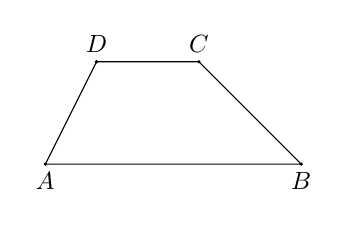
\begin{tikzpicture}[>=stealth,x=1cm,y=1cm,scale=0.65]
	\fill (0,0) circle (1pt) node[below]{$A$};
	\fill (5,0) circle (1pt) node[below]{$B$};
	\fill (3,2) circle (1pt) node[above]{$C$};
	\fill (1,2) circle (1pt) node[above]{$D$};
	\draw (0,0)--(5,0)--(3,2)--(1,2)--(0,0) ;
\end{tikzpicture}
}	
}
\end{ex}

\begin{ex}%[0X1B4-1]%[Dự án đề kiểm tra HKII NH22-23- Nguyễn Văn Sang]%[THPT Ngô Gia Tự - Phú Yên]
	Mẫu số liệu sau cho biết số ghế trống tại một rạp chiếu phim trong một tuần liên tiếp
	\begin{center}
	\begin{tabular}{|c|c|c|c|c|c|c|}
		\hline Thứ hai & Thứ ba & Thứ tư & Thứ năm & Thứ sáu & Thứ bảy & Chủ nhật \\
		\hline 16 & 17 & 16 & 22 & 9 & 3 & 2 \\
		\hline
	\end{tabular}
	\end{center}
	Khoảng tứ phân vị của mẫu số liệu này là
	\choice
	{$3$}
	{$17$}
	{\True $14$}
	{$22$}
	\loigiai{
		Sắp xếp các số liệu theo thứ tự không giảm, ta được
		$$2;3;9;16;16;17;22.$$
		\begin{itemize}
			\item Tứ phân vị.\\
			Vì cỡ mẫu là số lẻ nên trung vị mẫu là $16$.\\
			Tứ phân vị thứ hai là trung vị của mẫu số liệu đã cho nên $Q_2=16$.\\
			Tứ phân vị thứ nhất là trung vị của mẫu
			$$2, 3, 9.$$
			Do đó $Q_1=3$.\\
			Tứ phân vị thứ ba là trung vị của mẫu 
			$$16, 17, 22.$$
			Do đó $Q_3=17$.
			\item Khoảng tứ phân vị.\\
			Khoảng tứ phân vị là $\Delta_Q=Q_3-Q_1=17-3=14$.
		\end{itemize}
	}
\end{ex}

\begin{ex}%[X1Y3-4]%[Dự án đề kiểm tra HKII NH22-23- Nguyễn Văn Sang]%[THPT Ngô Gia Tự - Phú Yên]
	Cho bảng số liệu điểm bài kiểm tra môn toán của 45 học sinh lớp 10A ở một trường THPT
	\begin{center}
	\begin{tabular}{|l|c|c|c|c|c|c|c|}
		\hline Điểm & 2 & 5 & 6 & 7 & 8 & 9 & 10 \\
		\hline Số học sinh & 2 & 8 & 9 & 12 & 6 & 4 & 4 \\
		\hline
	\end{tabular}
\end{center}
	Tìm mốt của bảng số liệu trên.
	\choice
	{$4$}
	{$10$}
	{\True $7$}
	{$12$}
	\loigiai{
mốt của bảng số liệu là $7$.
}
\end{ex}

\begin{ex}%[0H3K1-4]%[Dự án đề kiểm tra HKII NH22-23- Nguyễn Văn Sang]%[THPT Ngô Gia Tự - Phú Yên]
	Trong mặt phẳng tọa độ $Oxy$, cho hai điểm $A(-1;-2)$, $B(5;0)$. Giao điểm của đường thẳng $AB$ với trục $Oy$ có tung độ là
	\choice
	{$-\dfrac{8}{5}$}
	{$-1$ }
	{$-\dfrac{3}{2}$}
	{\True $-\dfrac{5}{3}$}
	\loigiai{
Gọi $I(0;y)$ là giao điểm của đường thẳng $AB$ và trục $Oy$.\\
Ta có $\overrightarrow{AB}=(6;2)$ và $\overrightarrow{AI}=(1;y+2)$.\\
Vì $A$, $B$, $I$ thẳng hàng nên 
\begin{eqnarray*}
	\overrightarrow{AI}=k\cdot \overrightarrow{AB}&\Leftrightarrow& \heva{& 1=6k \\ & y+2=2k}\\
	&\Leftrightarrow& \heva{& k=\dfrac{1}{6} \\ & y=-\dfrac{5}{3}.}\\
\end{eqnarray*}
 Giao điểm của đường thẳng $AB$ với trục $Oy$ có tung độ là $y=-\dfrac{5}{3}$.
}
\end{ex}

\begin{ex}%[0X1B1-3]%[Dự án đề kiểm tra HKII NH22-23- Nguyễn Văn Sang]%[THPT Ngô Gia Tự - Phú Yên]
	Khi sử dụng máy tính bỏ túi, ta được $\sqrt{6}=2{,}449489743$. Giá trị gần đúng của $\sqrt{6}$ chính xác đến hàng phần trăm là
	\choice
	{\True $2{,}45$}
	{$2{,}44$}
	{$2{,}43$}
	{$2{,}40$}
	\loigiai{
 Giá trị gần đúng của $\sqrt{6}$ chính xác đến hàng phần trăm là$2{,}45$.
}
\end{ex}

\Closesolutionfile{ans}
%\begin{center}
%	\textbf{ĐÁP ÁN}
%	\inputansbox{10}{ans/ans}	
%\end{center}
\begin{center}
	\textbf{PHẦN 2 - TỰ LUẬN}
\end{center}

\begin{bt}%[0D1K3-5]%[Dự án đề kiểm tra HKII NH22-23- Nguyễn Văn Sang]%[THPT Ngô Gia Tự - Phú Yên]
	 Cho các tập hợp $A=(-7;6)$ và $B=[m-1;m+8]$.
	\begin{enumerate}
		\item Với $m=6$, xác định tập $B \backslash A$.
		\item Tìm tất cả các số thực $m$ để $A \cap B \neq \varnothing$.
	\end{enumerate}
\loigiai{
\begin{enumerate}
	\item Với $m=6$, ta được $B=[5;14]$.\\
	Khi đó $B \backslash A=[6;14]$.
	\item Tìm tất cả các số thực $m$ để $A \cap B \neq \varnothing$.\\
	Ta có $A\cap B=\varnothing \Leftrightarrow \hoac{&m+8 \leq -7 \\& m-1 \geq 6} \Leftrightarrow \hoac{&m \leq -15 \\& m \geq 7} \Leftrightarrow m \in (-\infty ;-15]\cup [7;+\infty)$.\\
	Vậy $A\cap B \neq \varnothing \Leftrightarrow m \in (-15;7)$.
\end{enumerate}	
}
\end{bt}

\begin{bt}%[0H1Y1-2]%[Dự án đề kiểm tra HKII NH22-23- Nguyễn Văn Sang]%[THPT Ngô Gia Tự - Phú Yên]
Cho $\sin \alpha=\dfrac{3}{5}$. với $90^{\circ}<\alpha<180^{\circ}$. Tính $\cos \alpha$ và $\tan \alpha$.
	\loigiai{
	Với $90^{\circ}<\alpha<180^{\circ}$ ta có
	\begin{itemize}
		\item $\cos \alpha=-\sqrt{1-\sin^2\alpha}=-\sqrt{1-\left(\dfrac{3}{5}\right)^2}=-\dfrac{4}{5}$.
		\item $\tan \alpha=\dfrac{\sin \alpha}{\cos \alpha}=\dfrac{\dfrac{3}{5}}{-\dfrac{4}{5}}=-\dfrac{3}{4}$.
	\end{itemize}
}
\end{bt}

\begin{bt}%[0H3G2-6]%[Dự án đề kiểm tra HKII NH22-23- Nguyễn Văn Sang]%[THPT Ngô Gia Tự - Phú Yên]
	\hfill
	\begin{enumerate}
		\item Cho tam giác $ABC$ có các đỉnh $A(2;2), B(5;1), C(-1;-2)$. Tìm tọa độ điểm $H$ là chân đường cao kẻ từ đỉnh $A$ lên cạnh $BC$.
		\item Cho tam giác $ABC$ đều cạnh $a$. Gọi $M$ là điểm trên $AC$ thỏa mãn biểu thức $T=MA^2+2MB^2$ nhỏ nhất. Tính độ dài đoạn thẳng $BM$.
	\end{enumerate}
	\loigiai{
	\begin{enumerate}
		\item Gọi $H(x;y)$ là chân đường cao kẻ từ đỉnh $A$ lên cạnh $BC$.\\
		Ta có 
		\begin{eqnarray*}
			&&\heva{& \overrightarrow{AH}\cdot \overrightarrow{BC}=0 \\ &\overrightarrow{BH},\overrightarrow{BC} \text{ cùng phương}}\\
			&\Leftrightarrow& \heva{& (x-2;y-2)\cdot(-6;-3)=0 \\ & (x-5;y-1)=k(-6;-3)}
			\\
			&\Leftrightarrow& \heva{&-6x+12-3y+6=0 \\ & x-5=-6k\\&y-1=-3k}
			\\
			&\Leftrightarrow& \heva{&-6x-3y=-18 \\ & x+6k=5\\&y+3k=1}
			\Leftrightarrow \heva{&x=3 \\ & y=0\\&k=\dfrac{1}{3}.}
		\end{eqnarray*}
		Vậy $H(3;0)$.
		\item Cho tam giác $ABC$ đều cạnh $a$. Gọi $M$ là điểm trên $AC$ thỏa mãn biểu thức $T=MA^2+2MB^2$ nhỏ nhất. Tính độ dài đoạn thẳng $BM$.
		\immini
		{
		Lấy $I$ là điểm trên đoạn thẳng $AB$ thoả mãn
$IA=2IB$.\\
Khi đó, $\overrightarrow{IA}+2\overrightarrow{IB}=\overrightarrow{0}$.\\

Ta có
\begin{eqnarray*}
	T&=&MA^2+2MB^2=\overrightarrow{MA}^2+2\overrightarrow{MB}^2=\overrightarrow{MI}+\overrightarrow{IA}^2+2\overrightarrow{MI}+\overrightarrow{IB}^2 \\ &=&3MI^2+IA^2+2IB^2+2\overrightarrow{MI}\overrightarrow{IA}+2\overrightarrow{IB}=3MI^2+IA^2+2IB^2.
\end{eqnarray*}
Vì $I$ là điểm cố định nên $IA^2+2IB^2$ là số không đổi.\\
Do đó $T$ nhỏ nhất khi $MI$ nhỏ nhất. Mà $M$ nằm trên $AC$ nên $M$ là hình chiếu vuông góc của $I$ trên cạnh $AC$.\\
Gọi $H$ là trung điểm của $AC$. Khi đó, $AM=\dfrac{2}{3}AH=\dfrac{1}{3}AC=\dfrac{a}{3}$.\\
Theo định lý cosin thì 
\begin{eqnarray*}
	BM^2&=&AB^2+AM^2-2AB\cdot AM\cdot \cos BAM\\
	    &=&a^2+\left(\dfrac{a}{3}\right)^2-2\cdot a\cdot \dfrac{a}{3}\cdot \cos 60^{\circ}=\dfrac{7}{9}a^2.
\end{eqnarray*}
Vậy $BM=\dfrac{a\sqrt{7}}{3}$.
		}
		{
		\begin{tikzpicture}[>=stealth,x=1cm,y=1cm,scale=1]
			\fill (0,0) coordinate (A) circle (1pt) node[below]{$A$};
			\fill (3,0) coordinate (B) circle (1pt) node[below]{$B$};
			\fill (1.5,2.6) coordinate (C) circle (1pt) node[above]{$C$};
			\fill (2,0)  coordinate (I) circle (1pt) node[below]{$I$};
			\fill (0.5,0.85)  coordinate (M) circle (1pt) node[left]{$M$};
			\coordinate (H) at ($(A)!1/2!(C)$); 
			\fill (H) circle (1pt) node[left]{$H$};
			\draw (A)--(B)--(C)--(A) (I)--(M)--(B)--(H);
			\draw (M)--++(-120:0.2)--++(-30:0.2)--++(60:0.2);
			\draw (H)--++(-120:0.2)--++(-30:0.2)--++(60:0.2);
		\end{tikzpicture}
		}
\end{enumerate}}
\end{bt}


